As pointed out earlier, the consistency of data stored in NVRAM is vulnerable to
crashes or power failures. Since NVRAM is directly attached to the processor
memory interface, there is no need to use techniques such as DMA to transfer a
modified page to external storage. This also means that a memory operation
solely relies on the CPU which usually gives no confirmation when that operation
completes. In this context, there are two major issues that threaten the
consistency of data written to NVRAM, namely out-of-order execution and deferred
write-back.

\paragraph{Out-Of-Order Execution}

When executing a program, processors fetch instructions on a consecutive manner.
Some instructions may inflict minimal latency, while others such as load
operations may delay further execution for hundreds of cycles. In an attempt to
optimize instruction throughput, individual instructions may be reordered. While
compilers may statically define promising orders, processors are able to reorder
instructions at runtime. This enables processors to optimize resource
utilization and hide latencies of time-consuming instructions. However, only
reorderings that do not violate data dependencies between instructions are
possible. While processors do prevent such conflicts, there are dependencies
that cannot be observed. For example, in order to mark a chunk of data as
durable in NVRAM, one might store a designated flag immediately after the
operation completed. With out-of-order execution it is possible that the flag is
written before the payload. This can lead to severe inconsistencies especially
when a crash prevents the chunk from being written.

A common method to counter this issue is to enforce memory order with memory
barriers (also fences) \cite{dulloor2014system, schwalb2016hyrise,
oukid2017data}. A memory barrier prevents the CPU from proceeding until all
prior memory operations have completed. Although a barrier does not directly
order its preceding instructions, it can be used to impose an order on separate
sequences of instructions. An example for a memory barrier is \code{sfence} on
x86 architectures. While this approach solves the initial problem, it has a
notable drawback. Memory barriers defeat the purpose of out-of-order execution.
As a result, CPU pipelines are likely to stall, hence reducing resource
utilization. Furthermore, store buffers are flushed leading to higher latencies
when accessing data of deferred store operations. Therefore, barriers can have
significant impact on runtime performance, unless used judiciously. With
\emph{epoch barriers} a similar approach has been proposed to address both order
and durability issues \cite{condit2009better}.

\paragraph{Deferred Write-Back}

In many modern processor architectures store operations may not  be immediately
lead to an update in main memory. This behaviour can be caused by intermediary
buffers such as memory order buffers, caches, and memory controller buffers.
While their individual purpose may vary, they all defer memory write-back
operations. This is a known vulnerability for consistency in NVRAM as the
mentioned buffers are volatile and deferred stores may be lost when power fails
\cite{condit2009better, oukid2017data}. In order to preserve consistency, it is
necessary to force write-back in all of these cases.

\begin{figure}[!ht]
    \centering
    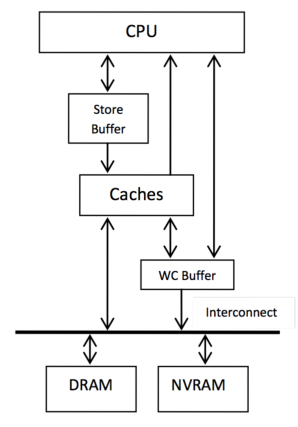
\includegraphics[scale=0.75]{figures/nvram-memory-subsystem.pdf}
    \caption{Architecture of memory subsystem \cite{bhandari2012implications}}
    \label{fig:memory-interface}
\end{figure}

% memory order buffers

In conjunction with instruction scheduling and cache coherency protocols a
memory order buffer may be present. It holds all loads and stores, with the
exception of non-temporal operations. In order to prevent a deferred write-back
through memory order buffers, their store buffers must be flushed. On x86
architectures this can be achieved with a store fence operation such as
\code{sfence}. As mentioned above, memory barriers carry a considerable
overhead. However, if memory barriers are already used for enforcing program
order, then flushing store buffers is a desirable side effect and incurs no
overhead.

% caches

Processor caches help avoid access latencies and reduce memory bus traffic for
frequently used data. A possible exception are non-temporal stores and data
chunks marked as uncacheable. Similar to memory order buffers, caches are
volatile so an abrupt power failure may lead to lost updates. The issue with
this is not that updates are lost but that it is unclear which updates are lost,
if any. The reason for this circumstance is the cache eviction policy trying to
compensate for typically narrow cache volume. Depending on policy, cache
content, and system load, a modified chunk may or may not be flushed to main
memory. An example of an application scenario where such behaviour is
unacceptable is transactions. Imagine an updating transaction $t1$ that commits
but is not evicted from cache. Then a transaction $t2$ based on the result of
$t1$ commits and gets evicted from cache. If the system crashes at this point,
$t2$'s result will be durable while $t1$'s initial update is lost.

\todo[inline]{Insert figure showing inconsistency due to crash}

\begin{lstlisting}
T1: r(A) w(A) c*   -- Cache ---------------------- (crash)
T2: -------------- r(A) w(B) c -- Cache -- RAM --- (crash)
\end{lstlisting}

An approach to prevent such inconsistencies is to disable caching for selected
memory regions but that could introduce considerable overhead for frequently
used data. A more popular approach is to evict cache lines programmatically
whenever necessary \cite{condit2009better, dulloor2014system, oukid2017data}. On
x86 architectures this can be done with the \code{clflush} or \code{clflushopt}
instructions. However, the problem with a simple cache line flush such as
\code{clflush} is that making a cache line durable may not always mean that is
should be evicted. In this regard, \code{clwb} compensates for this matter by
retaining the designated cache line \cite{kolli2016high}. Unfortunately, at the
time of this writing there is no evidence of a processor to implement this
instruction.

% memory controller queues

Once a cache line is flushed, it is propagated to the memory controller where it
is buffered in a write-back queue before being written onto the device. Again,
the problem is that such a buffer is usually volatile. This means that a power
failure could lead to lost updates to NVRAM. Even though residual power in DRAM
has been shown to be substantial, there is no reliable way to ensure a full
buffer flush \cite{halderman2008lest}. This circumstance has given rise to many
discussions in the past \cite{condit2009better, dulloor2014system,
kolli2016high}. Some authors proposed a designated instruction for flushing
write-back queues. An example is the meanwhile deprecated \code{pcommit},
formerly known as \code{pm\_wbarrier} \cite{dulloor2014system, oukid2015instant,
schwalb2015nvm_malloc, volos2017whisper}. Others have developed more general
mechanisms for preserving consistency in NVRAM that also address this issue
\cite{condit2009better, pelley2014memory}. The current state of affairs is
that platforms must provide a feature called ADR \cite{volos2017whisper}. It
works by exploiting the fact that even in case of a power failure there is
sufficient power to flush the write buffers of all memory controllers. For this
to work, the power supply unit has to detect a power failure and issue a signal
to all memory controllers. As a result, neither programmers nor processors need to worry about memory controller queues and no overhead is incurred.
